\documentclass[UTF8]{ctexart}
\ctexset { section = { format={\Large \bfseries } } }
\pagestyle{plain}
\usepackage{float}
\usepackage{amsmath}
\usepackage{amssymb}
\usepackage{listings}
\usepackage{graphicx}
\usepackage{xcolor}
\usepackage{geometry}
\geometry{a4paper,scale=0.8}
\usepackage{caption}
\captionsetup[figure]{name={Figure}}
\captionsetup[table]{name={Table}}

\lstset{tabsize=4,
language=R, %
frame=none,  %把代码用带有阴影的框圈起来
backgroundcolor=\color[RGB]{240,240,240},%背景
commentstyle=\ttfamily,
rulesepcolor=\color{red!20!green!20!blue!20},  %代码块边框为淡青色
keywordstyle=\color{blue},  %代码关键字的颜色为蓝色,粗体
showstringspaces=false,  %不显示代码字符串中间的空格标记
stringstyle=\ttfamily,  % 代码字符串的特殊格式
keepspaces=true,
breakindent=22pt,
numbers=left,  %左侧显示行号
stepnumber=1,
numberstyle=\scriptsize,  %行号字体用小号
basicstyle={\footnotesize\ttfamily},
showspaces=false,
flexiblecolumns=true,
breaklines=true,  %对过长的代码自动换行
breakautoindent=true,
breakindent=4em,
aboveskip=1em,  %代码块边框
fontadjust,
captionpos=t,
framextopmargin=1pt,framexbottommargin=1pt,abovecaptionskip=-9pt,belowcaptionskip=9pt,
xleftmargin=2em,xrightmargin=1em,  % 设定listing左右的空白
texcl=true,
% 设定中文冲突,断行,列模式,数学环境输入,listing数字的样式
extendedchars=false,columns=flexible,mathescape=false
numbersep=-1em,
morekeywords={in, TRUE, FALSE, filter, group, color, size}
}

\title{\textbf{Computational Statistics Homework 1}}
\author{吴嘉骜 21307130203}
\date{\today}

\begin{document}

\maketitle

\noindent
\section{ex 3.5}
\setlength{\parindent}{0pt}
A discrete random variable $X$ has probability mass function
\begin{table}[H]
    \centering
    \begin{tabular}{cccccc}
        $x$ & 0 & 1 & 2 & 3 & 4 \\
        \hline
        $p(x)$ & 0.1 & 0.2 & 0.2 & 0.2 & 0.3
    \end{tabular}
\end{table}
Use the inverse transform method to generate a random sample of size 1000
from the distribution of $X$. Construct a relative frequency table and compare
the empirical with the theoretical probabilities. Repeat using the R \texttt{sample}
function.\\
\textbf{Solution:}\\
First, we use the inverse transform method to generate the required random sample. We first calculate the cumulative distribution function of $X$:
\begin{equation*}
    F(x) = \begin{cases}
        0, & x < 0 \\
        0.1, & 0 \leq x < 1 \\
        0.3, & 1 \leq x < 2 \\
        0.5, & 2 \leq x < 3 \\
        0.7, & 3 \leq x < 4 \\
        1, & x \geq 4
    \end{cases}
\end{equation*}
Then we generate $u$ from $Unif(0, 1)$ 1000 times, and use the inverse of $F$ to transform the sample to the required distribution. If $u \in [0, 0.1]$, 
then $x = 0$; if $u \in (0.1, 0.3]$, then $x = 1$; if $u \in (0.3, 0.5]$, then $x = 2$; if $u \in (0.5, 0.7]$, then $x = 3$; if $u \in (0.7, 1]$, then $x = 4$. 
The R code and result are as follows:
\begin{lstlisting}
> # Inverse transform method
> n <- 1000
> p <- c(0.1, 0.2, 0.2, 0.2, 0.3)
> p_cdf <- cumsum(p)
> x <- rep(n,0)
> for(i in 1:n){
+   u <- runif(1)
+   x[i] <- sum(u>p_cdf)
+ }
> rbind(table(x)/n,p)
        0     1     2     3     4
    0.096 0.198 0.214 0.194 0.298
p   0.100 0.200 0.200 0.200 0.300
\end{lstlisting}
We can see that the empirical probabilities are very close to the theoretical probabilities.\\

Then we use the R \texttt{sample} function to generate the required random sample. The R code and result are as follows:
\begin{lstlisting}
> # Sample function
> n <- 1000
> p <- c(0.1, 0.2, 0.2, 0.2, 0.3)
> y <- sample(0:4, size=n, prob=p, replace=T)
> rbind(table(y) / n, p)
        0     1     2     3     4
    0.098 0.205 0.197 0.193 0.307
p   0.100 0.200 0.200 0.200 0.300
\end{lstlisting}


\section{ex 3.6}
Prove that the accepted variates generated by the acceptance-rejection sampling 
algorithm are a random sample from the target density $f_X$.\\
\textbf{Proof:}\\
Let $X$ be the random variable generated by the Acceptance-Rejection sampling algorithm, and $Y$ be the auxiliary random variable from density $g_Y$.
We assume that there exits a constant $c$ such that $f_X(t) \leq cg_Y(t)$ for all $t$ where $f_X(t) > 0$.\\
Let $U$ be a random variable from $Unif(0, 1)$, and $A$ be the set of accepted values $y$.\\
Given $Y = y$, the probability that $y$ is accepted is
\begin{equation*}
    P(A|Y=y) = P(U < \frac{f_X(y)}{cg_Y(y)}|Y=y) = \frac{f_X(y)}{cg_Y(y)}.
\end{equation*}
Then we have
\begin{equation*}
    P(A)=\int_{-\infty}^{\infty}P(A|Y=y)g_Y(y)dy = \int_{-\infty}^{\infty}\frac{f_X(y)}{cg_Y(y)}g_Y(y)dy = \frac{1}{c}.
\end{equation*}
By Bayes' theorem, we have
\begin{equation*}
    g_{Y|A}(y|A) = \frac{P(A|Y=y)g_Y(y)}{P(A)} = \frac{f_X(y)}{cg_Y(y)} \cdot g_Y(y) \cdot \frac{1}{1/c} = f_X(y).
\end{equation*}
Therefore, the accepted variates generated by the Acceptance-Rejection sampling algorithm are a random sample from the target density $f_X$.


\section{ex 3.9}
The rescaled Epanechnikov kernel is a symmetric density function
\begin{equation*}
    f_e(x) = \frac{3}{4} (1 - x^2), \quad |x| \leq 1.
\end{equation*}
Devroye and Gy$\ddot{o}$rfi give the following algorithm for simulation
from this distribution. Generate iid $U_1, U_2, U_3$ $\sim$  Uniform(−1, 1). If $|U_3| \geq |U_2|$ and $|U_3| \geq |U_1|$, 
deliver $U_2$; otherwise deliver $U_3$.
Write a function to generate random variates from $f_e$, and construct the histogram density
estimate of a large simulated random sample.\\
\textbf{Solution:}\\
The R code is as follows:
\begin{lstlisting}
# Rescaled Epanechnikov kernel
rREpan <- function(n){
    u1 <- runif(n, -1, 1)
    u2 <- runif(n, -1, 1)
    u3 <- runif(n, -1, 1)
    x <- rep(n, 0)
    for(i in 1:n){
    if(abs(u3[i]) >= abs(u2[i]) && abs(u3[i]) >= abs(u1[i]))
        x[i] <- u2[i]
    else
        x[i] <- u3[i]
    }
    return(x)
}

x <- rREpan(10000)
hist(x,prob=T)
y <- seq(-1, 1, 0.001)
fe <- 0.75 * (1 - y^2)
lines(y,fe)
\end{lstlisting}
The histogram density estimate of a 10000-size random sample together with the theoretical density is as follows:
\begin{figure}[H]
    \centering
    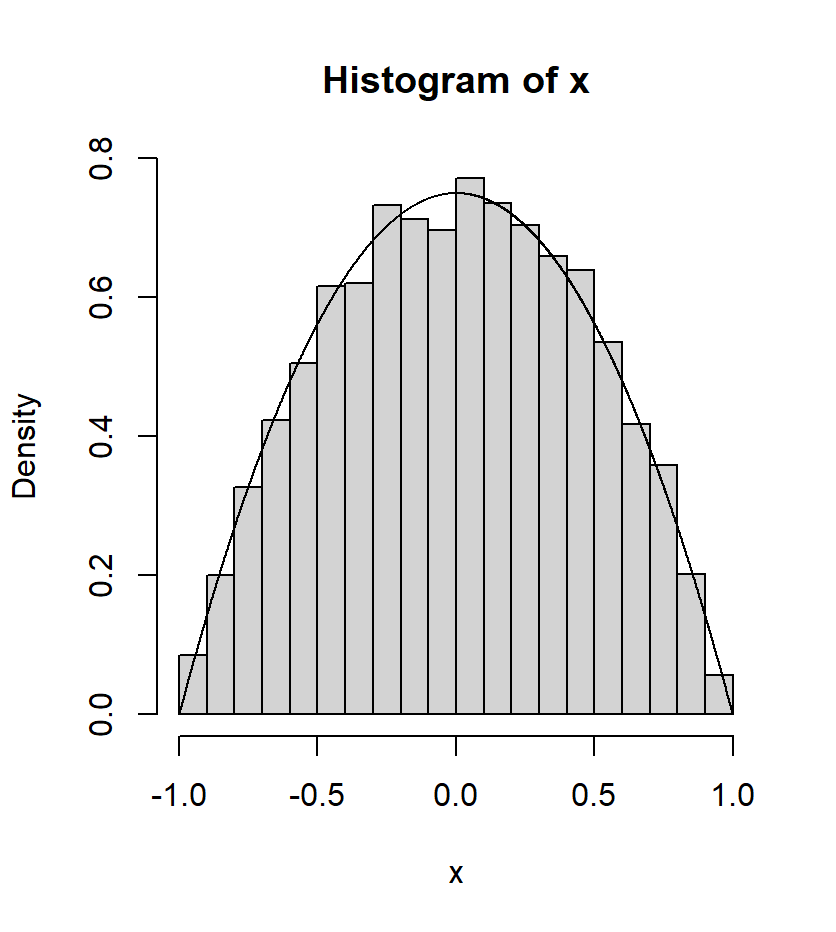
\includegraphics[width=0.4\textwidth]{ex3-9.png}
    \caption{Histogram of a Rescaled Epanechnikov kernel sample}
\end{figure}

\section{ex 3.10}
Prove that the algorithm given in Exercise 3.9 generates variates from the density $f_e$.\\
\textbf{Proof:}\\
The algorithm equvalently generates iid $V_1, V_2, V_3$ $\sim$ Uniform(0, 1), and choose the first or second order statistic (not the largest) $V$ with equal probability $\frac{1}{2}$, then
let $X = \pm V$ with probability $\frac{1}{2}$ respectively.\\
Notice that $V$ is a mixture of $V_{(1)}$ and $V_{(2)}$, where $V_{(1)}$ and $V_{(2)}$ are the first and second order statistics of $V_1, V_2, V_3$.
So the cumulative distribution function of $V$ is $ F_V(v) = \frac{1}{2}F_{V_{(1)}}(v) + \frac{1}{2}F_{V_{(2)}}(v)$.\\
As is known, the pdf of $V_{(k)}$ is $f_{V_{(k)}}(v) = k \tbinom{n}{k} v^{k-1}(1-v)^{n-k}$, $v \in (0, 1)$.\\
So the pdf of $V_{(1)}$ is $f_{V_{(1)}}(v) = 3(1-v)^2$, and the pdf of $V_{(2)}$ is $f_{V_{(2)}}(v) = 6v(1-v)$, and the pdf of
$V$ is $f_V(v) = \frac{1}{2}f_{V_{(1)}}(v) + \frac{1}{2}f_{V_{(2)}}(v) = \frac{3}{2}(1-v^2)$.\\
Therefore, the pdf of $X$ is $f_X(x) = \frac{1}{2}f_V(x) = \frac{3}{4}(1-x^2)$, which is the density $f_e$.

\section{ex 3.12}
Simulate a continuous Exponential-Gamma mixture. Suppose that the rate
parameter $\Lambda$ has Gamma(r, $\beta$) distribution and $Y$ has Exp($\Lambda$) distribution.
That is, $(Y|\Lambda = \lambda) \sim f_Y (y|\lambda) = \lambda e^{-\lambda y}$. Generate 1000 random observations
from this mixture with $r = 4$ and $\beta = 2$.\\
\textbf{Solution:}\\
The R code is as follows:
\begin{lstlisting}
# Exponential-Gamma mixture
n <- 1000
r <- 4
beta <- 2
lambda <- rgamma(n,r,beta)
x <- rexp(n,lambda)
\end{lstlisting}

\section{ex 3.13}
It can be shown that the mixture in Exercise 3.12 has a Pareto distribution
with cdf
\begin{equation*}
    F (y) = 1 - \left(\frac{\beta}{\beta+y}\right)^{r}, \quad y \geq 0.
\end{equation*}
(This is an alternative parameterization of the Pareto cdf given in Exercise
3.3.) Generate 1000 random observations from the mixture with $r = 4$ and
$\beta = 2$. Compare the empirical and theoretical (Pareto) distributions by graphing
the density histogram of the sample and superimposing the Pareto density curve.\\
\textbf{Solution:}\\
The probability density function of Pareto distribution is
\begin{equation*}
    f(y) = \frac{r\beta^{r}}{(y+\beta)^{r+1}}, \quad y \geq 0.
\end{equation*}
The R code is as follows:
\begin{lstlisting}
# Exponential-Gamma mixture and Pareto dist
n <- 1000
r <- 4
beta <- 2
lambda <- rgamma(n,r,beta)
x <- rexp(n,lambda)
hist(x,prob=T)
y <- sort(x)
f_pareto=r * beta^r / (beta + y)^(r + 1)
lines(y,f_pareto)
\end{lstlisting}
The histogram density estimate of a 1000-size random sample together with the theoretical density is as follows:
\begin{figure}[H]
    \centering
    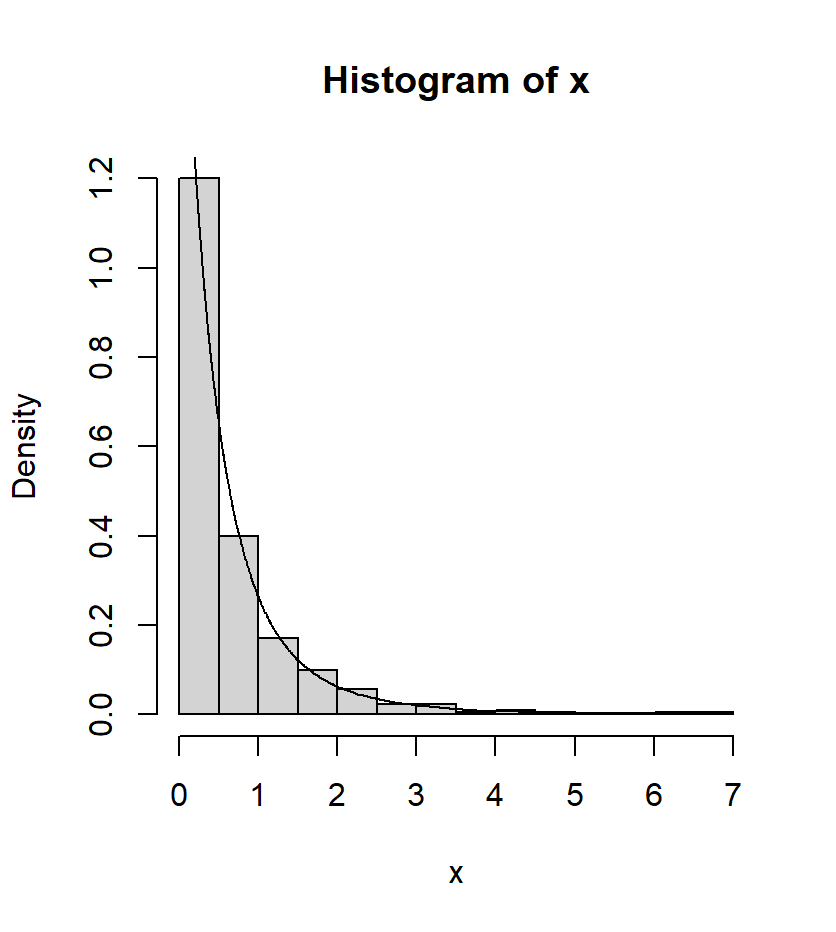
\includegraphics[width=0.4\textwidth]{ex3-13.png}
    \caption{Histogram of an Exponential-Gamma mixture sample}
\end{figure}
From the figure we can see that the histogram density estimate is close to the theoretical density.

\section{ex 3.14}
Generate 200 random observations from the 3-dimensional multivariate normal 
distribution having mean vector $\mu = (0, 1, 2)$ and covariance matrix
\begin{equation*}
    \Sigma = \begin{bmatrix}
        1.0 & -0.5 & 0.5 \\
        -0.5 & 1.0 & -0.5 \\
        0.5 & -0.5 & 1.0
    \end{bmatrix}.
\end{equation*}
using the Choleski factorization method. Use the R \texttt{pairs} plot to graph an
array of scatter plots for each pair of variables. For each pair of variables,
(visually) check that the location and correlation approximately agree with
the theoretical parameters of the corresponding bivariate normal distribution.\\
\textbf{Solution:}\\
The R code and result are as follows:
\begin{lstlisting}
> rmvn_Chol <- function(n,mu,sigma){
    +   d <- length(mu)
    +   CT <- chol(sigma)
    +   Z <- matrix(rnorm(n*d),n,d)
    +   X <- Z%*%CT + matrix(mu,n,d,byrow=T)
    +   return(X)
    + }
> sigma <- matrix(c(1, -0.5, 0.5, -0.5, 1, -0.5, 0.5, -0.5, 1), 3, 3)
> mu <- c(0, 1, 2)
> x <- rmvn_Chol(200, mu, sigma)
> colMeans(x)
[1] 0.03386865 0.96643718 2.07497880
> cor(x)
            [,1]       [,2]       [,3]
[1,]  1.0000000 -0.5018619  0.4559275
[2,] -0.5018619  1.0000000 -0.5306230
[3,]  0.4559275 -0.5306230  1.0000000
> pairs(x)
\end{lstlisting}
\begin{figure}[H]
    \centering
    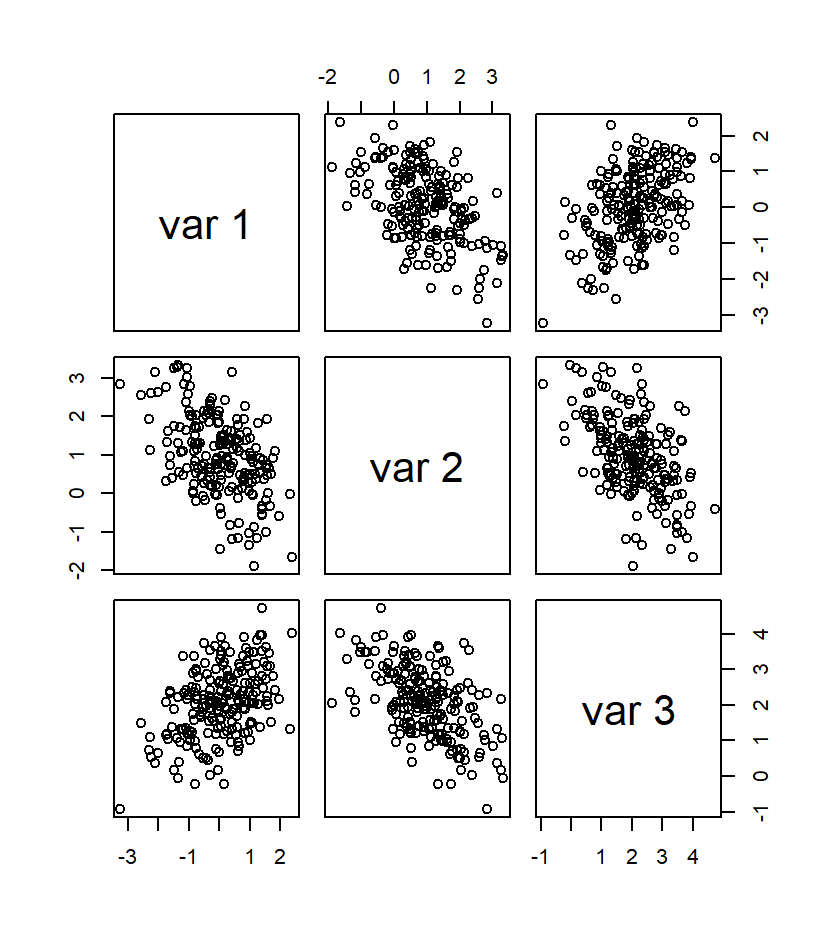
\includegraphics[width=0.4\textwidth]{ex3-14.png}
    \caption{Pairs plot of a 3-dimensional multivariate normal distribution}
\end{figure}
From the sample mean and sample correlation we can see that the generated sample is close to the specified parameters.\\
From the \texttt{pairs} plot we can see that the centers of the three variables are approximately $(0, 1, 2)$, and the correlations approximately agree with $\Sigma$.\\

\end{document}